% =====================================================================
%  gTAO-Net Article 2 — controlled diagnostic of multimodal fusion
%  Rebuilt 2026-11-04 from the surviving artifacts (results JSON, Kaggle
%  sources, Q&A pack, review). Every number is generated by
%  analysis/stats.py + analysis/tables.py from gtao-net/results/*.json.
%  Build: latexmk main.tex   (output in build/)
%  Target: Intelligent Systems with Applications (Elsevier, elsarticle)
% =====================================================================
\documentclass[preprint,11pt]{elsarticle}
\usepackage[T1]{fontenc}
\usepackage[utf8]{inputenc}
\usepackage{amsmath,amssymb}
\usepackage{booktabs}
\usepackage{array}
\usepackage{graphicx}
\usepackage{xcolor}
\usepackage{tikz}
\usetikzlibrary{arrows.meta,positioning,calc,fit,backgrounds}
\usepackage{pgfplots}
\pgfplotsset{compat=1.18}
\usepackage[margin=2.0cm,top=2.0cm,bottom=2.0cm]{geometry}
\usepackage{xurl}
\usepackage[hidelinks]{hyperref}
\usepackage{microtype}
\usepackage{titlesec}
\titlespacing*\section{0pt}{6pt}{3pt}
\titlespacing*\subsection{0pt}{4pt}{2pt}
\setlength{\parskip}{2pt}
\setlength{\parindent}{10pt}

\newcommand{\qwk}{QWK}
% Placeholder for a value or verdict that comes from the v2 (nested) Kaggle runs.
% Every \pending must be gone before submission: grep -n pending sections/*.tex
\newcommand{\pending}[1]{\textcolor{red}{\textbf{[#1]}}}
% Protocol switch, written by analysis/tables.py: \nestedtrue for the v2 results
% (nested early stopping), \nestedfalse for v1.
\newif\ifnested
\nestedtrue

% Our numbers quoted in the prose of the DAiSEE comparison (written by analysis/comparison.py).
% \cmptesttrue: our comparison rows score the official Test partition (protocol P1-Test).
\newif\ifcmptest
\newcommand{\cmpBestName}{face stream, CORAL}
\newcommand{\cmpBestQWK}{0.043}
\newcommand{\cmpBestQWKsd}{0.013}
\newcommand{\cmpBestAcc}{50.4}
\newcommand{\cmpMajAcc}{51.8}
\newcommand{\cmpNScored}{1{,}638}
\cmptesttrue

% Full-corpus numbers quoted in the prose (written by analysis_v3/paper_fullcorpus.py).
% written by analysis_v3/paper_fullcorpus.py -- do not edit
\newcommand{\fcPersons}{57}
\newcommand{\fcSessions}{483}
\newcommand{\fcWindows}{35{,}649}
\newcommand{\fcComplete}{28{,}926}
\newcommand{\fcShareHigh}{15.1}
\newcommand{\fcSharePerson}{13}
\newcommand{\fcShareClass}{20}
\newcommand{\fcShareSession}{49}
\newcommand{\fcExpPrior}{0.372}
\newcommand{\fcMomentPrior}{0.378}
\newcommand{\fcBestSingleQWK}{0.116}
\newcommand{\fcBestSingleCI}{[0.077, 0.158]}
\newcommand{\fcBestFusionQWK}{0.100}
\newcommand{\fcFusionDiff}{$-$0.016}
\newcommand{\fcFusionDiffCI}{[$-$0.052, $+$0.020]}
\newcommand{\fcFusionP}{0.37}
\newcommand{\fcFusionsAbove}{0 of 24}
\newcommand{\fcWithinSessionMax}{0.051}
\newcommand{\fcPartialR}{0.074}
\newcommand{\fcClassmateStream}{face}
\newcommand{\fcClassmateP}{0.14}
\newcommand{\fcLeakRandAcc}{65.4}
\newcommand{\fcLeakRandQWK}{0.342}
\newcommand{\fcLeakPersonAcc}{57.2}
\newcommand{\fcLeakPersonQWK}{0.122}
\newcommand{\fcMajority}{54.4}
\newcommand{\fcSearchPaperAcc}{58.0}
\newcommand{\fcSearchRichAcc}{58.9}
\newcommand{\fcSearchCropAcc}{57.5}
\newcommand{\fcSearchCropQWK}{0.192}
\newcommand{\fcSearchMajority}{52.0}
\newcommand{\fcCropAccGain}{4.9}
\newcommand{\fcCropAccCI}{[+2.3, +7.2]}
\newcommand{\fcCtxNoneQWK}{0.161}
\newcommand{\fcCtxGruQWK}{0.165}
\newcommand{\fcCtxBiQWK}{0.167}
\newcommand{\fcLogoOwnAcc}{53.9}
\newcommand{\fcLogoOwnQWK}{0.085}
\newcommand{\fcLogoClassQWK}{0.103}
\newcommand{\fcPgOwnQWK}{0.173}
\newcommand{\fcPgClassQWK}{0.316}
\newcommand{\fcLeakClassDiff}{$+$0.143}
\newcommand{\fcLeakClassCI}{[$+$0.080, $+$0.204]}
\newcommand{\fcLogoDrop}{$-$0.103}
\newcommand{\fcLogoDropCI}{[$-$0.170, $-$0.038]}
\newcommand{\fcLogoSeedZeroQWK}{0.070}
\newcommand{\fcProbeHalfAcc}{74.2}
\newcommand{\fcProbeHalfQWK}{0.605}
\newcommand{\fcPersistHalfAcc}{72.3}
\newcommand{\fcPersistHalfQWK}{0.604}
\newcommand{\fcProbeHalfGain}{1.8}
\newcommand{\fcProbeHalfGainCI}{[$+$1.2, $+$2.5]}
\newcommand{\fcProbeOneAcc}{70.0}
\newcommand{\fcProbeOneQWK}{0.536}
\newcommand{\fcPersistOneAcc}{68.9}
\newcommand{\fcPersistOneQWK}{0.554}
\newcommand{\fcProbeOneGain}{1.1}
\newcommand{\fcProbeOneGainCI}{[$+$0.1, $+$2.2]}
\newcommand{\fcProbeLongAcc}{65.8}
\newcommand{\fcProbeLongQWK}{0.417}
\newcommand{\fcPersistLongAcc}{62.9}
\newcommand{\fcPersistLongQWK}{0.431}
\newcommand{\fcProbeLongGain}{2.9}
\newcommand{\fcProbeLongGainCI}{[$+$1.5, $+$4.2]}
\newcommand{\fcSensorsOnlyAcc}{55.5}
\newcommand{\fcSensorsOnlyQWK}{0.048}
\newcommand{\fcMajorityAll}{50.4}
\newcommand{\fcEncBaseAcc}{55.5}
\newcommand{\fcEncBaseQWK}{0.050}
\newcommand{\fcEncResAcc}{55.3}
\newcommand{\fcEncResQWK}{0.044}
\newcommand{\fcEncDinoAcc}{54.7}
\newcommand{\fcEncDinoQWK}{0.017}
\newcommand{\fcEncExprAcc}{55.2}
\newcommand{\fcEncExprQWK}{0.016}
\newcommand{\fcSelfExtAcc}{45.4}
\newcommand{\fcSelfExtQWK}{0.224}
\newcommand{\fcSelfPersistHalfAcc}{43.3}
\newcommand{\fcSelfPersistHalfQWK}{0.195}
\newcommand{\fcSelfFullHalfAcc}{49.2}
\newcommand{\fcSelfFullHalfQWK}{$-$0.029}
\newcommand{\fcExtPersistHalfAcc}{70.5}
\newcommand{\fcExtPersistHalfQWK}{0.581}

\journal{Intelligent Systems with Applications}

\begin{document}
\begin{frontmatter}

\title{Does Multimodal Fusion Help Classroom Attention Estimation?\\
A Controlled Diagnostic of Gated Ordinal Fusion on DIPSER, DAiSEE and EngageNet}

\author[uit]{Zakaria Makhkhas\corref{cor}}
\ead{zakaria.makhkhas@uit.ac.ma}
\author[crmef]{Amal Rifai}
\author[uit]{Abdelalim Sadiq}
\cortext[cor]{Corresponding author.}
\affiliation[uit]{organization={Computer Science Research Laboratory, Faculty of Sciences, Ibn Tofail University},
  city={K\'enitra}, country={Morocco}}
\affiliation[crmef]{organization={Centre R\'egional des M\'etiers de l'\'Education et de la Formation (CRMEF)},
  city={Rabat}, country={Morocco}}

\begin{abstract}
Multimodal attention systems assume that fusing more data streams improves recognition. We test this with gTAO-Net, one model in which each design choice is a switch: gated versus mean-pooled fusion, a linear input-to-head link, modality dropout, and three ordinal objectives (CORAL, a CORE-style hybrid and a soft multi-rater target). All streams share a training-free Tchebichef-moment front-end. On a DIPSER slice of 20 students, none of the 24 fusion configurations exceeds the best single stream (face mesh with the soft target, QWK $0.256\pm0.068$, against $0.124\pm0.071$ for the best fusion), and the gate is not significantly different from mean pooling ($p=0.68$). Only the input-to-head link ($p=0.002$) and the soft target ($p=0.023$) help, and fusion yields no meaningful gain on DAiSEE or EngageNet. On the full DIPSER release (\fcPersons{} students, \fcWindows{} windows) the fusion result replicates (\fcFusionsAbove{} fusions above it), but the sensor signal is weak (best QWK \fcBestSingleQWK) and largely shared by the class. Hyper-parameter search, richer and local moments, a face crop, frozen pretrained face encoders, and temporal and class context do not improve on it. A label probe every 32\,s raises accuracy to \fcProbeHalfAcc\% on an unseen class, but repeating the probe already gives \fcPersistHalfAcc\%. The evaluation protocol has a larger effect than any of these choices: the same model obtains QWK \fcLeakRandQWK{} on random windows, \fcLeakPersonQWK{} on held-out students and \fcLogoOwnQWK{} on a held-out class, while its accuracy remains close to the majority rate (\fcMajority\%).
\end{abstract}

\begin{keyword}
student attention \sep multimodal fusion \sep ordinal regression \sep multi-rater labels \sep Tchebichef moments \sep evaluation protocol \sep data leakage \sep DIPSER
\end{keyword}

\end{frontmatter}

\section{Introduction}
\label{sec:intro}

Automatic estimation of student attention is a long-standing objective of learning analytics and affective computing~\cite{whitehill2014faces,chango2022datafusionmmla}. Most systems analyse webcam recordings of individual learners, such as DAiSEE~\cite{gupta2016daisee} and EngageNet~\cite{singh2023engagenet}, and combine several modalities (face, landmarks, head pose and, when available, physiology) through attention or gating~\cite{baltrusaitis2019multimodal,arevalo2017gated,tran2026ordinal}. The underlying premise is that each stream contributes information and that learned fusion weights it appropriately.

This premise is rarely tested in isolation. Reported gains are typically accuracy differences on a single split, obtained with different backbones and protocols for fused and single-stream systems. The multimodal learning literature shows that joint models can underperform their best unimodal branch, because modalities learn at different rates and a dominant modality suppresses the others~\cite{wang2020makes,peng2022balanced}. Whether this holds for classroom attention, where labels are noisy, ordinal and imbalanced, has not been measured.

DIPSER~\cite{marquezcarpintero2025dipser} makes such a test possible. It provides real classroom sessions with per-student cameras and smartwatches, and each window is rated by several annotators. Since a controlled diagnostic requires hundreds of trainings, we encode every stream with discrete Tchebichef moments~\cite{mukundan2001tchebichef}. They require no training and keep each downstream model small, so the study remains affordable without a GPU cluster.

This paper is a diagnostic rather than a state-of-the-art claim. It addresses six questions: (Q1) whether any fusion exceeds the best single stream; (Q2) whether a learnable gate differs from mean pooling; (Q3) whether a linear input-to-head link helps; (Q4) which ordinal objective performs best under rater disagreement; (Q5) whether the answers transfer to DAiSEE and EngageNet; and (Q6) whether they hold on the full DIPSER release, and how much of a reported score depends on the evaluation protocol.

The contributions are as follows. (i) We provide a controlled fusion benchmark on DIPSER, with nested epoch selection and released results for all 495 fits. (ii) We use a shared training-free moment front-end for four modalities, with at most 2.1\,M parameters per model. (iii) We report a negative result with its mechanism: no fusion exceeds the best single stream, and the gate collapses to one stream. (iv) We identify two components that help, the linear link and the soft multi-rater target, and prove that the latter reduces to CORAL under a single label. (v) We provide a transfer study on DAiSEE and EngageNet. (vi) We report a study of the full DIPSER release in which, apart from one exploratory search, success criteria were fixed before each run. It shows that the sensor signal is largely shared by the class, that seven attempts to improve on it fail, and that the evaluation split changes QWK four-fold while accuracy barely changes.

\section{Related work}
\label{sec:related}

\textbf{Engagement recognition.} Engagement recognition grew out of facial-expression analysis~\cite{whitehill2014faces} and was then extended by webcam datasets: DAiSEE~\cite{gupta2016daisee} provides four-level labels for short clips, and EngageNet~\cite{singh2023engagenet} provides about 11{,}300 ten-second clips of 127 participants; the EmotiW challenges made engagement prediction a shared task~\cite{dhall2018emotiw,dhall2020emotiw}. On DAiSEE, reported accuracy has risen from about 59\% to 73\%, but almost all results are single top-1 accuracies on the official test split, without seed variation or QWK. Because DAiSEE is dominated by its two highest levels, accuracy hides the failure on minority classes: where it can be derived, recall for the lowest level is between 0 and 0.25~\cite{abedi2021resnettcn,abedi2024affectordinal,abedi2025supervised,gothwal2025vibednet}. Ordinal structure is exploited only occasionally~\cite{abedi2024affectordinal,abedi2025supervised}. DIPSER~\cite{marquezcarpintero2025dipser} is, to our knowledge, the only public dataset with per-student video, landmarks, head pose and smartwatch signals from real classrooms, rated by external annotators and by the students. Liu et al.~\cite{liu2025attention} also evaluate attention recognition on DIPSER, and CORE-Net~\cite{tran2026ordinal} recognises ordinal engagement from several modalities on another classroom dataset; our earlier work provided a single-stream Tchebichef baseline on DIPSER~\cite{makhkhas2026ordinal}. On DIPSER, a wearable-sensor model does not improve on the training mean~\cite{fragkiadakis2026fairness}. Splits that share subjects inflate scores~\cite{saeb2017need}, personal baselines are often omitted~\cite{demasi2017meaningless}, and for self-rated engagement in video learning, carrying the last rating forward outperforms a sensor model~\cite{leng2026edugage}.

\textbf{Fusion, ordinal objectives and moments.} Fusion strategies range from early fusion by feature concatenation to late fusion by averaging decisions~\cite{baltrusaitis2019multimodal}; gated units learn input-dependent weights~\cite{arevalo2017gated}, and modality dropout improves robustness to missing streams~\cite{neverova2016moddrop}. Joint training can nevertheless perform worse than the best unimodal model, because networks overfit faster and modalities learn at different rates~\cite{wang2020makes}, a dominant modality suppresses weaker gradients~\cite{peng2022balanced}, and transformers degrade when a modality is absent~\cite{ma2022robust}. CORAL decomposes a $K$-level ordinal problem into $K-1$ rank-consistent binary tasks~\cite{cao2020coral}, and CORE-Net combines cross-entropy, a squared earth mover's distance and a neighbour penalty~\cite{tran2026ordinal}. Multi-rater labels can be voted, aggregated by expectation--maximisation~\cite{dawid1979em} or retained as distributions~\cite{geng2016ldl}. Discrete Tchebichef moments provide compact and numerically stable descriptors~\cite{mukundan2001tchebichef}.

\section{Datasets and task}
\label{sec:data}

\textbf{DIPSER slice.} We use session D1 of DIPSER~\cite{marquezcarpintero2025dipser}, segmented into non-overlapping 4-s windows. Four external raters and the student (self-report) mark attention on a 1--5 scale as change points. For each rater, a window takes the latest annotation at or before its midpoint, which gives up to five votes. The levels are collapsed into three ordinal classes (low $=\{1,2\}$, medium $=\{3\}$, high $=\{4,5\}$). The hard label is the most frequent vote (ties go to the lower class), and the soft label is the vector of vote fractions $\bar p\in\Delta^{2}$. The streams are the student's webcam frame (640$\times$480), MediaPipe face mesh with iris points (478$\times$3)~\cite{kartynnik2019facemesh,grishchenko2020attentionmesh}, head pose (three angles) and eight smartwatch channels. The webcam frame is used whole and therefore also shows the classroom and often other students. We retain the name \emph{face stream} for consistency with earlier work, although it is not a face crop (Section~\ref{sec:fc-crop}). The slice contains 2{,}959 windows from 40 student-sessions (20 students, two sessions each), with class counts [1{,}447, 1{,}502, 10]. Physiology is available in 52.9\% of windows. All slice experiments use the complete-window population, in which every stream exists: 1{,}566 windows, 23 student-sessions and counts [679, 880, 7].

\textbf{Full DIPSER release.} Section~\ref{sec:fullcorpus} uses every labelled student-session of DIPSER, extracted with the same code: \fcPersons{} students in three class groups (20, 21 and 16 students), \fcSessions{} student-sessions in 27 class sessions, and \fcWindows{} windows with counts [12{,}306, 17{,}964, 5{,}379] (\fcShareHigh\% high). Of these windows, \fcComplete{} have every stream. Each session is rated by four external raters, drawn from a pool of five, and by the student.

\textbf{DAiSEE and EngageNet.} DAiSEE~\cite{gupta2016daisee} contains webcam clips with four levels; requiring all three visual streams leaves 7{,}919 clips from 101 subjects, with counts [60, 425, 4{,}136, 3{,}298] and six frames per clip. Its official splits are subject-disjoint. EngageNet~\cite{singh2023engagenet} is described with a subject-independent split. The release we used, however, contains 31{,}512 frame-level samples from 91 subjects with four levels and counts [5{,}780, 4{,}140, 6{,}632, 14{,}960], and in it the training, validation and test splits share subjects (our check); we therefore use only subject-grouped folds. Mesh and pose were extracted for 98.4\% of samples and missing streams are zero-filled; since samples are single frames, temporal moments carry no motion.

\textbf{Metric.} The primary metric is the quadratic weighted kappa (QWK)~\cite{cohen1968weighted}. It equals 1 for perfect agreement and 0 for chance or constant prediction, and it weights an error by the square of its distance, which suits imbalanced ordinal labels. Accuracy is reported for comparability, together with the majority-class rate.

\section{The instrument: gTAO-Net}
\label{sec:instrument}

gTAO-Net (gated Tchebichef Attention Ordinal network) implements each design choice as a switch. For a window $x=\{x_k\}_{k=1}^{S}$ with $S$ streams, the logits are
\begin{equation}
  \ell(x)=h\big(F(T(x))+G(x)\big),
\end{equation}
where $T$ denotes the stream towers, $F$ the fusion operator, $G$ an optional global link and $h$ the ordinal head (Fig.~\ref{fig:arch}).

\begin{figure}[!htbp]
\centering
\resizebox{0.85\linewidth}{!}{%
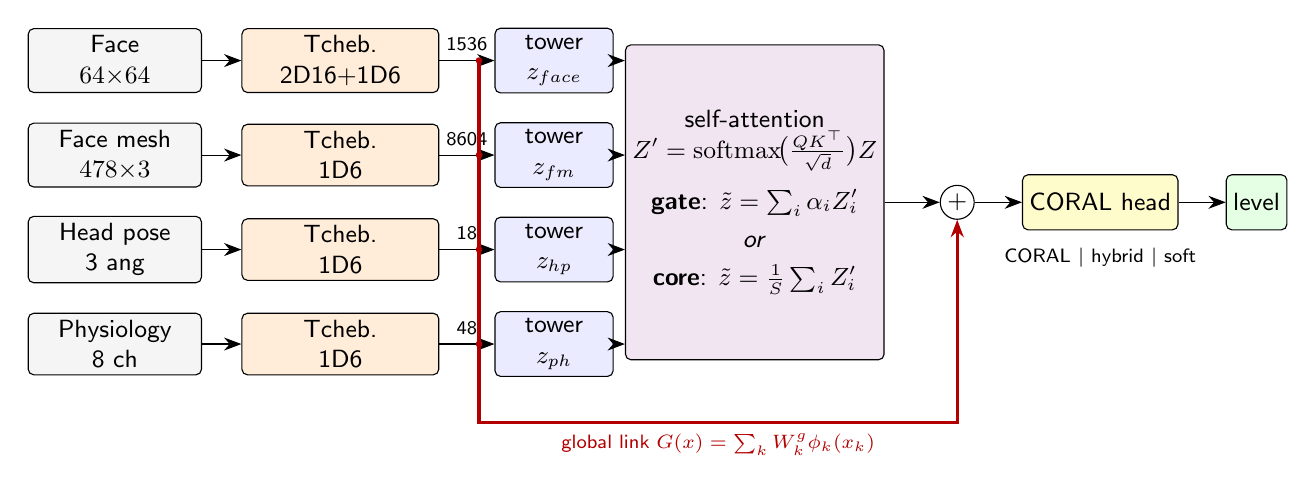
\begin{tikzpicture}[
  font=\sffamily\small, >={Stealth[length=2.2mm]},
  box/.style={draw, rounded corners=2pt, minimum height=7mm, align=center, inner sep=2.5pt},
  inp/.style={box, fill=gray!8, minimum width=22mm},
  mom/.style={box, fill=orange!15, minimum width=25mm},
  tow/.style={box, fill=blue!8, minimum width=15mm},
  op/.style={box, fill=violet!10},
  ]
  \foreach \n/\lab/\enc/\dim [count=\i] in
    {face/{Face\\$64{\times}64$}/ {2D16+1D6}/1536,
     fm/{Face mesh\\$478{\times}3$}/{1D6}/8604,
     hp/{Head pose\\3 ang}/{1D6}/18,
     ph/{Physiology\\8 ch}/{1D6}/48} {
    \node[inp] (in\n) at (0,-1.2*\i) {\lab};
    \node[mom, right=5mm of in\n] (m\n) {Tcheb.\\\enc};
    \node[tow, right=7mm of m\n] (t\n) {tower\\$z_{\n}$};
    \draw[->] (in\n) -- (m\n);
    \draw[->] (m\n) -- node[above, font=\sffamily\scriptsize]{\dim} (t\n);
  }
  \node[op, minimum height=40mm, minimum width=28mm, right=9mm of $(tfm)!0.5!(thp)$] (fuse)
    {self-attention\\$Z'=\mathrm{softmax}\!\big(\tfrac{QK^\top}{\sqrt d}\big)Z$\\[2mm]
     \textbf{gate}: $\tilde z=\sum_i \alpha_i Z'_i$\\[1mm] \emph{or}\\[1mm]
     \textbf{core}: $\tilde z=\tfrac1S\sum_i Z'_i$};
  \foreach \n in {face,fm,hp,ph} \draw[->] (t\n.east) -- (fuse.west |- t\n.east);
  \node[draw, circle, inner sep=1pt, right=7mm of fuse] (plus) {$+$};
  \node[box, fill=yellow!20, right=6mm of plus] (head) {CORAL head};
  \node[box, fill=green!10, right=6mm of head] (out) {level};
  \draw[->] (fuse) -- (plus); \draw[->] (plus) -- (head); \draw[->] (head) -- (out);
  \coordinate (lk) at ($(inph.south)+(0,-6mm)$);
  \foreach \n in {face,fm,hp,ph} {
    \coordinate (tap\n) at ($(m\n.east)!0.72!(t\n.west)$);
    \fill[red!70!black] (tap\n) circle (1.2pt);
  }
  \draw[very thick, red!70!black] (tapface) -- (tapph);
  \draw[->, very thick, red!70!black] (tapph) -- (tapph |- lk) -| node[pos=0.25, below, font=\sffamily\scriptsize] {global link $G(x)=\sum_k W^{g}_k\phi_k(x_k)$} (plus.south);
  \node[below=1mm of head, font=\sffamily\scriptsize] {CORAL $|$ hybrid $|$ soft};
\end{tikzpicture}}
\caption{gTAO-Net: fixed Tchebichef front-ends $\phi_k$, stream towers, gate or core fusion, an optional linear global link, and a CORAL head trained with one of three objectives.}
\label{fig:arch}
\end{figure}

\textbf{Front-ends and towers.} Each stream is a short per-frame sequence. Face-stream frames are converted to grey $64\times64$ images and projected on the 2-D Tchebichef basis of order 16~\cite{mukundan2001tchebichef}; every coefficient, landmark coordinate, angle and physiological channel is then projected in time on the 1-D basis of order 6. This yields fixed vectors of 1{,}536 (face), 8{,}604 (mesh), 18 (pose) and 48 (physiology) dimensions, which are computed once and cached; no front-end parameter is learned. One transform family thus serves all four modalities, so adding a stream requires choosing a moment order rather than training an encoder~\cite{makhkhas2026ordinal}. Each tower computes $z_k=\mathrm{LN}(W_2\,\mathrm{GELU}(W_1\phi_k))\in\mathbb{R}^{64}$ (hidden size 128). Single-stream baselines consist of one tower followed by the head.

\textbf{Fusion.} The stacked summaries $Z$ pass through one self-attention step with bias-free query and key projections, $Z'=\mathrm{softmax}(QK^\top/\sqrt{d})Z$. The \emph{gate} maps $Z'$ through a two-layer MLP $g$ to weights $\alpha=\mathrm{softmax}(g(\mathrm{vec}\,Z'))$ and returns $\tilde z=\sum_i\alpha_iZ'_i$; these weights allow it to discard a stream. The \emph{core} variant, following CORE-Net~\cite{tran2026ordinal}, returns the mean $\tilde z=S^{-1}\sum_iZ'_i$ and cannot discard a stream. Modality dropout~\cite{neverova2016moddrop} zeroes each tower output with probability 0.2 during training, independently per sample and stream and without rescaling; the global link receives the unmasked inputs.

\textbf{Global link and objectives.} The global link $G(x)=\sum_kW^{g}_k\phi_k(x_k)$ is linear and bias-free, so its gradient reaches the input in two steps, as in a residual shortcut~\cite{he2016deep}. The CORAL head~\cite{cao2020coral} computes $\ell_k=w^\top u+b_k$ with $u=\tilde z+G(x)$. Three objectives are compared: \textbf{CORAL}, a binary cross-entropy between $\sigma(\ell_k)$ and $\mathbf{1}[y>k]$; \textbf{hybrid}, inspired by CORE-Net~\cite{tran2026ordinal}, which adds to the cross-entropy on the implied class probabilities 0.5 times the CORAL loss and 0.1 times a cross-entropy to a neighbour-smoothed target (0.7 on the true class and 0.15 on each neighbour, renormalised at the extremes); unlike CORE-Net, it has no earth mover's term and gives some probability to neighbouring classes instead of penalising it; and \textbf{soft}, a binary cross-entropy against $t_k=1-\sum_{j\le k}\bar p_j$.

\noindent\textbf{Proposition.} If $\bar p$ is one-hot at $y$, then $t_k=\mathbf{1}[y>k]$ and the soft objective equals CORAL. Consequently, soft and CORAL are identical on the single-label datasets DAiSEE and EngageNet (confirmed bit-identical in the logs), and on DIPSER any difference between them arises from rater disagreement alone.

\section{Protocol}
\label{sec:protocol}

\textbf{Design.} On the DIPSER slice we cross fusion $\in\{$gate, core$\}$, link $\in\{$on, off$\}$, dropout $\in\{$on, off$\}$ and objective $\in\{$CORAL, hybrid, soft$\}$, giving 24 cells, to which we add eight single-stream baselines and one permuted-label control. With five folds and three seeds this amounts to 495 fits. The control is core fusion with link and dropout on and the CORAL objective, trained on labels permuted across the population; it must satisfy $|\mathrm{QWK}|\le0.10$. DAiSEE uses the same 24 cells and three single-stream baselines (16 distinct fusion models, since soft and CORAL are identical). Because of Kaggle time limits, EngageNet uses a disclosed subset (three single streams, gate and core with link on and dropout off, and the control; 90 fits).

\textbf{Splits.} The main protocol (P2) is a subject-grouped five-fold cross-validation in which no grouping unit appears in both training and test folds; QWK is computed on the pooled out-of-fold predictions. On the slice the grouping unit is the student-session, so the three students with complete windows in both sessions may contribute one session to training and the other to testing (5--20\% of scored windows, depending on the seed); Section~\ref{sec:threats} reports a re-evaluation on person-disjoint windows. From Section~\ref{sec:fullcorpus} onwards, folds group persons. For DAiSEE, protocol P1 trains on the official training subjects not present in Validation and tests on Validation (1{,}429 clips); P1-Test retrains the best P1 single-stream and fusion models, selected on Validation, on Train and Validation and scores them once on Test.

\textbf{Training and statistics.} Models are trained with Adam~\cite{kingma2015adam} (learning rate $3\times10^{-3}$, batch 32, gradient clipping at 1.0) for up to 40 epochs, with early stopping after eight epochs without improvement (not before epoch 9). Epoch selection is nested: 20\% of the training-fold subjects form an inner validation set, and the checkpoint with the best inner QWK is applied once to the outer fold. Seeds fix the folds, inner split, initialisation and sample order. Reference points are the majority predictor (QWK $=0$) and the leave-one-rater-out agreement of 0.230~\cite{makhkhas2026ordinal}, which measures rater agreement rather than an upper bound. Factorial contrasts compare matched configurations that differ in a single factor, using a two-sided Wilcoxon signed-rank test~\cite{wilcoxon1945} on configuration-level means (12 pairs for link, gate and dropout; 8 for the objectives); per-seed tests are reported as secondary.

\section{Results on the DIPSER slice and transfer}
\label{sec:results}

\subsection{Fusion versus the best single stream (Q1)}
Supplementary Table~S1 lists all DIPSER configurations. The best single stream is face mesh with the soft target (QWK $0.256\pm0.068$). The best fusion (gate, link on, dropout off, soft) reaches $0.124\pm0.071$ and the best core fusion $0.113\pm0.073$. On identical folds, the best fusion falls short of the best single stream by $0.327$, $0.046$ and $0.021$ for the three seeds (mean $0.131$); only 1 of 72 seed-level fusion results exceeds the corresponding best single stream, and 14 of the 24 configurations score at or below zero. Only the mesh stream carries signal (QWK $0.256$, against $0.003$ for the face stream, $0.002$ for physiology and $0.002$ for head pose), and the permuted-label control stays at $0.009\pm0.018$. Decision-level voting over the four single-stream predictions performs no better ($0.011\pm0.047$ and $0.006\pm0.028$ for soft and CORAL streams).

\subsection{Gate, global link and dropout (Q2, Q3)}
The gate is one-hot (weight $\ge0.98$ on one stream) in 108 of 180 gated fits (60\%) and selects the mesh stream in only 41 of them. Gate and core fusion do not differ significantly (gate better in 7 of 12 pairs, median difference $-0.009$, $p_{\text{cfg}}=0.68$; Table~\ref{tab:contrasts}); the same holds on DAiSEE ($p=0.46$ under P1, $0.95$ under P2). The global link improves DIPSER QWK in 10 of 12 pairs (median $+0.076$, $p=0.002$). At initialisation it makes the gradient reaching the first tower layers 12--132 times larger, although these single-seed probes do not establish the mechanism. On DAiSEE the effect reverses: the link improves 0 of 8 pairs under P1 and 1 of 8 under P2 (median $-0.046$ and $-0.024$; $p=0.008$ and $0.016$), probably because it gives the head direct access to high-dimensional, low-signal inputs. Modality dropout has no reliable effect (8 of 12 pairs, median $-0.016$, $p=0.62$).

\begin{table}[!htbp]
\centering
\caption{Paired contrasts. Wins: pairs in which the first level has the higher mean QWK. Med./Mean $\Delta$: median and mean per-seed QWK differences. $p_{\text{cfg}}$: Wilcoxon test on configuration-level means (primary); $p_{\text{seed}}$: on per-seed differences (secondary).}
\label{tab:contrasts}
\footnotesize
\setlength{\tabcolsep}{3pt}
\begin{tabular}{llccccc}
\toprule
Contrast & Data & Wins & Med. $\Delta$ & Mean $\Delta$ & $p_{\text{cfg}}$ & $p_{\text{seed}}$ \\
\midrule
\csname @@input\endcsname tables/contrasts.tex
\bottomrule
\end{tabular}
\end{table}

\subsection{Ordinal objectives (Q4)}
The soft target outperforms CORAL in 7 of 8 fusion pairs (median $+0.062$, $p=0.023$) and the hybrid objective in 7 of 8 ($+0.117$, $p=0.016$). By the proposition of Section~\ref{sec:instrument}, the difference between soft and CORAL can arise only from rater disagreement. On person-disjoint windows the soft target still wins 6 of 8 pairs, but no longer significantly ($p=0.078$), so we regard this gain as weak evidence only. For single streams it raises mesh from $0.092$ to $0.256$ and the face stream from $-0.163$ to $0.003$. Zeroing one stream at inference harms both fusion types, most strongly the mesh stream for the gate ($-0.129$) and the face stream for core fusion ($-0.111$). On the high level (7 windows), recall is 0.00 for the best single stream and 0.19 for the best fusion, which strongly over-predicts it; most errors are one level off (81--99\%).

\subsection{Transfer to DAiSEE and EngageNet (Q5)}
Fusion yields no meaningful gain beyond the best single stream on DAiSEE ($+0.010$ under P2, $-0.001$ under P1) and trails it on EngageNet (gate $0.170$ against mesh $0.366$; Table~S3). The permuted controls remain near zero ($0.024$ and $0.035$). The informative stream differs between datasets: mesh leads on DIPSER and EngageNet, whereas on DAiSEE the face (P1, $0.093$) and head pose (P2, $0.050$) lead and all QWK values remain below $0.10$ because of class imbalance. On the official DAiSEE test set, the best single stream (face, CORAL, selected on Validation) obtains QWK $0.043\pm0.013$ at 50.4\% accuracy, and the best fusion $0.044\pm0.018$, whereas the majority predictor reaches 51.8\% (Table~\ref{tab:comparison}). Because published studies report no QWK and score a different set of clips, the table positions approaches rather than ranking them.

\begin{table}[!htbp]
\centering
\caption{DAiSEE four-class results on the official test set. Published: single reported figures. Ours: mean over 3 seeds (P1-Test). $^\ast$Derived from the published confusion matrix; n.r.: not reported.}
\label{tab:comparison}
\footnotesize
\setlength{\tabcolsep}{3pt}
\begin{tabular}{llccc}
\toprule
Method & Test clips & Acc.\,\% & Recall 0 & QWK \\
\midrule
DFSTN~\cite{liao2021dfstn} & n.r. & 58.84 & n.r. & n.r. \\
ResNet+TCN~\cite{abedi2021resnettcn} & 1{,}784 & 63.9 & 0.00$^\ast$ & n.r. \\
Ordinal TCN~\cite{abedi2024affectordinal} & 1{,}784 & 67.4 & 0.25$^\ast$ & n.r. \\
Contrastive ordinal~\cite{abedi2025supervised} & 1{,}784 & 67.32 & 0.00 & n.r. \\
ViBED-Net~\cite{gothwal2025vibednet} & n.r. & 73.43 & 0.25 & n.r. \\
Majority & 1{,}638 & 51.8 & 0.00 & 0.000 \\
gTAO-Net, best single stream & 1{,}638 & 50.4 & 0.00 & $0.043\pm0.013$ \\
gTAO-Net, best fusion & 1{,}638 & 50.2 & 0.00 & $0.044\pm0.018$ \\
\bottomrule
\end{tabular}
\end{table}

\textbf{Computational cost.} All 495 DIPSER fits train in 24 minutes on a Kaggle GPU and in an estimated 15--18 minutes on a laptop CPU, so the GPU brings no speed-up for models of 1.12--2.07\,M parameters (Supplementary Table~S2). Tchebichef encoding takes 0.6\,ms per window.

\section{The full DIPSER release (Q6)}
\label{sec:fullcorpus}

On the full release, all folds group persons, success criteria were fixed before each run unless stated otherwise, and all numbers are produced by Kaggle notebooks.

\subsection{Replication of the fusion result}
\label{sec:fc-fusion}
The factorial grid was rerun with standardised inputs, person-grouped folds and three seeds. The fusion result replicates: \fcFusionsAbove{} fusion configurations exceed the best single stream (face mesh, QWK \fcBestSingleQWK, 95\% CI \fcBestSingleCI; best fusion \fcBestFusionQWK; difference \fcFusionDiff{} \fcFusionDiffCI, $p=\fcFusionP$). All streams are, however, considerably weaker than on the slice, on which 59\% of the label variance lay between the 20 students, so that models could score by recognising which students tend to be attentive.  The agreement with changes \emph{within} a student-session is small (correlation $\le\fcWithinSessionMax$ for every stream), and no stream outperforms a control model trained on the label of a \emph{classmate} at the same moment (closest: \fcClassmateStream{} stream, $p=\fcClassmateP$). The sensors therefore capture mainly what the class is doing rather than what the individual student is doing.

\subsection{Structure of the labels}
\label{sec:fc-labels}
Of the label variance, \fcSharePerson\% lies between students, \fcShareClass\% between class sessions and \fcShareSession\% between student-sessions; attention is thus mainly a property of a lesson, and of a student within it, rather than as a stable trait. Two label-only references, which use no sensor but cannot be deployed because they read other students' labels, quantify this. The mean label of the other students in the same class session yields QWK \fcExpPrior, and the labels of the other students at the same 4-s moment yield \fcMomentPrior. Both are about twice the best sensor model.

\subsection{Attempts to improve the sensor model}
\label{sec:fc-limits}
Table~\ref{tab:fc-tests} summarises the attempts; every comparison is paired on the same students. \textbf{Search and richer moments.} A Bayesian search (Optuna, TPE) over streams, moment orders, model family (MLP or gradient-boosted trees), size, learning rate, class weights and head was evaluated on a fixed person-disjoint split with 13 test students, scored once with three seeds. It reaches \fcSearchPaperAcc\% test accuracy (majority \fcSearchMajority\%); moments re-extracted at higher orders ($24\times24$ spatially, 12 temporally) yield a non-significant \fcSearchRichAcc\%, and the search itself selects low orders (spatial 6--8, temporal 5--7).

\textbf{Face crop and moment families.}
\label{sec:fc-crop}
Inspection of the raw data showed that the DIPSER face stream used here and in our earlier work~\cite{makhkhas2026ordinal} is the whole webcam frame resized to $64\times64$. We therefore constructed a face crop from the per-frame face box in the DIPSER metadata (square, 10\% margin; frames without a detected face become blank images, so that face visibility itself is encoded). The crop was encoded with five discrete orthogonal moment families: Tchebichef, Hahn ($\alpha=\beta=4$) and Krawtchouk centred on the face, the eyes and the mouth. Unlike Tchebichef moments, Krawtchouk and Hahn moments are local and concentrate on a region of the image. A self-test confirmed that the whole-frame Tchebichef moments recomputed by the new pipeline equal the original features in all 35{,}374 comparable windows. The crop raises accuracy by \fcCropAccGain{} points \fcCropAccCI{} over the whole frame but does not significantly change QWK. No family outperforms Tchebichef under the predefined rule, which required a Holm-corrected gain in both an accuracy-tuned and a QWK-tuned search; the best family, Hahn, gains $+0.036$ in the latter (Holm $p=0.13$) and $+0.010$ in the former.

\textbf{Temporal and class context.} Because raters mark change points, consecutive windows usually share a label. A causal recurrent model (GRU) reading the student's preceding windows nevertheless leaves QWK unchanged (\fcCtxNoneQWK{} for isolated windows, \fcCtxGruQWK{} with the past and \fcCtxBiQWK{} for an offline bidirectional model). Adding the sensor features of the other students at the same moment, without their labels, does not significantly improve QWK on a class unseen during training (\fcLogoOwnQWK{} to \fcLogoClassQWK).

\textbf{Pretrained face encoders.} To test whether the moment front-end is the limit, we added frozen pretrained encoders of the face crop to the sensor features (mean and standard deviation of the frame embeddings of up to eight crops per window): ResNet-18~\cite{he2016deep}, DINOv2~\cite{oquab2024dinov2} and an expression network trained for emotion and engagement~\cite{savchenko2022hsemotion}. On a held-out class the sensor features give \fcEncBaseAcc\% and QWK \fcEncBaseQWK; adding an encoder gives QWK \fcEncResQWK, \fcEncDinoQWK{} and \fcEncExprQWK{} respectively, none significantly different (Table~\ref{tab:fc-tests}; the third encoder was run after the first two results were known).

\begin{table}[!htbp]
\centering
\caption{Attempts to improve performance on the full release. $\Delta$QWK: second condition minus first, paired on the same students (person bootstrap, 95\% CI); two-sided $p$, Holm-adjusted within the moment families and within the encoders. Phase: label in the released plan; explor.: no predefined criterion.}
\label{tab:fc-tests}
\footnotesize
\setlength{\tabcolsep}{2.5pt}
\begin{tabular}{lcccccc}
\toprule
Comparison & Phase & Rule & $\Delta$QWK & 95\% CI & $p$ & Helps \\
\midrule
\csname @@input\endcsname tables/fullcorpus_tests.tex
\bottomrule
\end{tabular}
\end{table}

\subsection{Tracking with sparse label probes}
\label{sec:fc-probe}
Since sensors alone fail, we tested a different task: the consensus label of a student is revealed at a probe every 32\,s, 1\,min or 2.5\,min, and the windows in between are predicted causally on a held-out class (rules fixed in advance; Table~S4). With a probe every 32\,s, a model of the probe labels and the sensors reaches \fcProbeHalfAcc\% accuracy and QWK \fcProbeHalfQWK, and \fcProbeOneAcc\% and \fcProbeOneQWK{} with one probe per minute, against \fcSensorsOnlyAcc\% and \fcSensorsOnlyQWK{} for sensors alone. Repeating the last probe (persistence), however, already gives \fcPersistHalfAcc\% and \fcPersistHalfQWK{} (\fcPersistOneAcc\% and \fcPersistOneQWK{} per minute): the sensors add \fcProbeHalfGain{} points of accuracy \fcProbeHalfGainCI{} and no QWK. This agrees with the carry-forward result for self-rated engagement in video learning~\cite{leng2026edugage} and extends it to an in-person classroom with multi-rater labels. The probe above is the consensus label. With the student's own self-report as the probe and the external raters as the target, persistence gives only \fcSelfPersistHalfAcc\% and QWK \fcSelfPersistHalfQWK{} at 32\,s, because self-reports agree poorly with the raters (QWK \fcSelfExtQWK); the result therefore requires observer-quality probes.

\subsection{Effect of the evaluation protocol}
\label{sec:fc-protocol}
Table~\ref{tab:fc-protocol} reports two experiments, each of which keeps the model fixed and changes only what the test set shares with the training set. With random windows, the windows of a student fall on both sides of the split, often seconds apart, and the model obtains \fcLeakRandAcc\% accuracy and QWK \fcLeakRandQWK; with whole students held out it obtains \fcLeakPersonAcc\% and \fcLeakPersonQWK{} (majority \fcMajority\%). Holding out a whole class lowers a second model from QWK \fcPgOwnQWK{} to \fcLogoOwnQWK{} (paired difference for seed 0: \fcLogoDrop{} \fcLogoDropCI), which shows that part of what is learned is specific to the lessons seen in training. The effect is largest when class features are used: with students held out, they appear to raise QWK from \fcPgOwnQWK{} to \fcPgClassQWK{} (\fcLeakClassDiff{} \fcLeakClassCI), because the classmates' labels at the same moment are in the training set and the class features allow the model to retrieve them. On an unseen class this gain is lost. Across the splits that hold out students or classes, accuracy remains within a few points of the majority rate (\fcLogoOwnAcc--\fcLeakPersonAcc\% against \fcMajority\%), whereas QWK decreases four-fold from random windows to held-out classes.

\begin{table}[!htbp]
\centering
\caption{The same model under different splits (full release, complete windows, pooled out-of-fold, majority accuracy \fcMajority\%). A: model of the hyper-parameter search (3 seeds); B: window-level MLP on all streams including the face crop (3 seeds; student-grouped: 1 seed); B$'$: B with the classmates' sensor features.}
\label{tab:fc-protocol}
\footnotesize
\setlength{\tabcolsep}{3pt}
\begin{tabular}{lllcc}
\toprule
Model & Split & Shared with training set & Acc.\,\% & QWK \\
\midrule
\csname @@input\endcsname tables/fullcorpus_protocol.tex
\bottomrule
\end{tabular}
\end{table}

\section{Discussion}
\label{sec:discussion}

Fusion yields no meaningful gain over the best single stream on any of the three datasets or on the full DIPSER release (at most $+0.010$ QWK, on DAiSEE). This agrees with accounts of multimodal failure~\cite{wang2020makes,peng2022balanced}: the gate collapses to one stream chosen by the optimisation rather than by how informative it is, and mean pooling weakens the single informative stream with uninformative ones. The components that help concern optimisation and supervision rather than fusion: the global link gives the head direct access to all inputs, and the soft target exploits the rater distribution and yields the best single model on the slice.

The full release changes the interpretation of the slice. On the slice, models appeared useful because they ranked 20 students; with 57 students, labels vary mainly between lessons, and the sensor signal is largely shared by the class. Neither richer or local moments, nor a face crop, nor pretrained face encoders, nor temporal or class context finds a student-specific signal, so the limitation lies in how little the per-student streams convey about labels that vary with the lesson, rather than in the encoder.  Each relaxation of the split introduces a leak: the same student a few seconds apart, classmates in the same lesson, and classmates' labels retrieved through class features. Accuracy hides all three, because it remains close to the majority rate.

\textbf{Recommendations.} (1) Report the best single-stream baseline under the same protocol as any fusion model. (2) With multiple raters, train on the vote distribution rather than the majority vote. (3) Interpret one-hot gates as stream selection, not fusion. (4) Do not transfer components across datasets without testing them, since the link helps on DIPSER but harms on DAiSEE. (5) For imbalanced ordinal labels, base conclusions on QWK and report accuracy together with the majority rate. (6) For claims about classrooms, hold out whole classes, since person-grouped folds still share lessons and, with class-level features, leak classmates' labels. (7) Report label-only references alongside the majority class; here, the other students of the same lesson give QWK \fcExpPrior. (8) When earlier labels of the same student are available, report label persistence~\cite{demasi2017meaningless}.

\subsection{Threats to validity}
\label{sec:threats}
On the slice, folds group student-sessions rather than persons; re-evaluating every run on person-disjoint windows leaves the main findings unchanged (no fusion above the best stream; gate versus core $p=0.79$; link 10 of 12 pairs, $p=0.021$; best stream $0.213$, best fusion $0.109$), but the soft-target gain is no longer significant ($p=0.078$). Nested selection removes selection bias but trains on 80\% of the fold subjects, so absolute values are not comparable with the earlier non-nested version~\cite{cawley2010overfitting}. Only complete windows are used, which removes 47\% of the slice and 19\% of the full release. The slice contains seven high-attention windows, and the mean fusion gap is driven by one seed. The face stream of the slice experiments is the whole webcam frame; Section~\ref{sec:fc-crop} tests a true crop. The full-release attempts used fixed model families (MLP, gradient-boosted trees, GRU); the face encoders were frozen, so we conclude that moment features, pretrained embeddings and context do not help, not that an encoder fine-tuned on classroom data could not. Leave-one-class-out uses only three folds, so its estimates are noisy.

\section{Conclusion}
\label{sec:conclusion}

Using one instrumented model and a nested protocol, we find that multimodal fusion does not improve classroom attention estimation. On a DIPSER slice, no fusion configuration exceeds face mesh with the soft target ($0.256$ against $0.124$), the gate does not differ from mean pooling, and only the input-to-head link and the soft target help; fusion also brings no gain on DAiSEE and EngageNet. On the full DIPSER release the fusion result replicates, but the per-student signal is weak and largely shared by the class, and hyper-parameter search, richer and local moments, a face crop, frozen pretrained face encoders, and temporal and class context fail to improve it. The evaluation split has a larger effect than any modelling choice: one model obtains QWK \fcLeakRandQWK{} on random windows, \fcLeakPersonQWK{} on held-out students and \fcLogoOwnQWK{} on a held-out class, with accuracy near the \fcMajority\% majority rate. Sparse probes of the raters' label raise accuracy above 70\%, but label persistence explains almost all of this gain, and self-report probes do not reproduce it. Classroom attention systems should therefore be evaluated on held-out classes, with QWK and label-only references. Future work will fine-tune face encoders and evaluate them on held-out classes.

\section*{Data and code availability}
DIPSER~\cite{marquezcarpintero2025dipser}, DAiSEE~\cite{gupta2016daisee} and EngageNet~\cite{singh2023engagenet} are public. Per-seed results, out-of-fold predictions and analysis scripts: \url{https://github.com/mks-zakaria/gtao-net}. Training code runs as public Kaggle notebooks: DIPSER \url{https://www.kaggle.com/code/zakariamakhas/gtao-net-dipser-grid-v2-nested-early-stopping}, DAiSEE \url{https://www.kaggle.com/code/zakariamakhas/gtao-net-daisee-v2-nested-early-stopping}, EngageNet \url{https://www.kaggle.com/code/zakariamakhas/gtao-net-engagenet-v2-nested-early-stopping}. The repository includes an independent verification script that recomputes every reported number from the raw predictions. The full-release analyses of Section~\ref{sec:fullcorpus} run as Kaggle notebooks, and every statistic is recomputed from their outputs by a separate notebook. \pending{Make these notebooks public and list their URLs here (never the data-extraction notebooks, which contain access credentials).}


\renewcommand{\bibfont}{\footnotesize}
\setlength{\bibsep}{0pt}
\bibliographystyle{elsarticle-num}
\bibliography{references}
\end{document}
